\documentclass{article}
\usepackage{
    xcolor,
    hyperref,
    geometry,
    multicol,
    enumitem,
    graphicx
}
\hypersetup{
    colorlinks,
    linkcolor={green!50!black},
    citecolor={red!50!black},
    urlcolor={blue!80!black}
}
\geometry{margin=1in}
\graphicspath{{./images/}}


\title{CSC 805 - Data Visualization\\\large Visualization Project - Phase 2}
\author{Jijeong Lee, Parth Panchal, Mark Kim}
\date{\today}

\begin{document}
\maketitle


%%%%%%%%%%%%%%%%%%%%%%%%%%%%%%%%%%%%%%%%%%%%%%%%%%%%
% WIREFRAME
%%%%%%%%%%%%%%%%%%%%%%%%%%%%%%%%%%%%%%%%%%%%%%%%%%%%
\section*{Wireframe}

%%%%%%%%%%%%%%%%%%%%%%%%%%%%%%%%%%%%%%%%%%%%%%%%%%%%
% TREE
%%%%%%%%%%%%%%%%%%%%%%%%%%%%%%%%%%%%%%%%%%%%%%%%%%%%
The visualization will be organized with a home page and five visualization
pages as can be shown in Figure \ref{fig:tree}.  The first page will be our
landing page, with the second page being the overview of the data we will be
presenting. The following page will display regional popularity information, followed by EV adoption trends and charging infrastructure details. The final page will provide an in-depth comparison of EV adoption with traditional fuel options.

\begin{figure}[h]
    \centering
    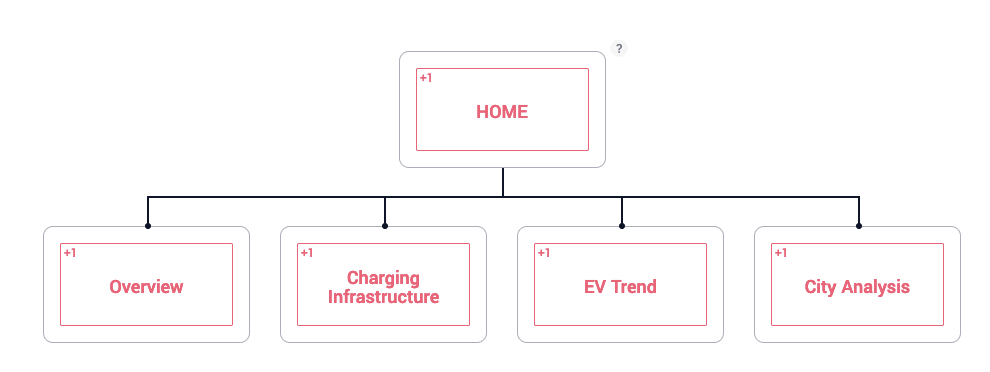
\includegraphics[scale=0.4]{Tree.png}
    \caption{Page Organization Tree}
    \label{fig:tree}
\end{figure}

%%%%%%%%%%%%%%%%%%%%%%%%%%%%%%%%%%%%%%%%%%%%%%%%%%%%
% HOME
%%%%%%%%%%%%%%%%%%%%%%%%%%%%%%%%%%%%%%%%%%%%%%%%%%%%
Our home page shown in Figure \ref{fig:home} will contain a short
description of our data, our visualizations, and direct the user to the
information they are seeking.  Finally, the home page will let the user know the
purpose of our visualization.
\begin{figure}[h]
    \centering
    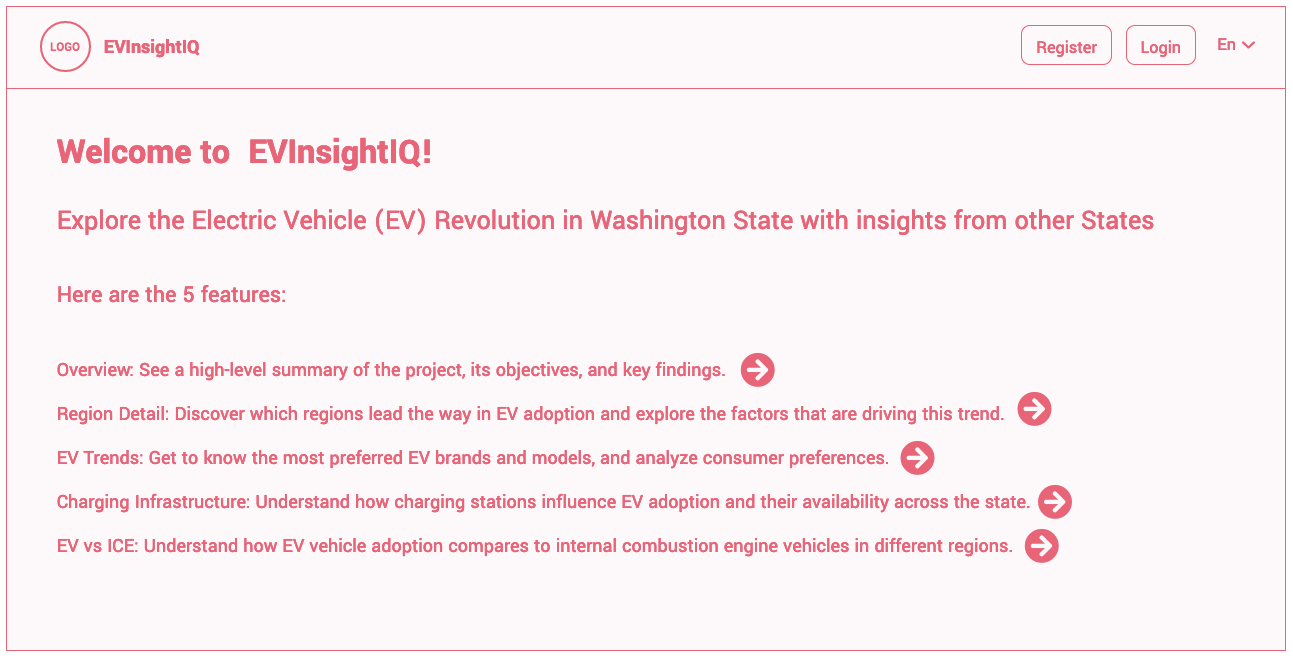
\includegraphics[scale=0.25]{Home}
    \caption{Home Page}
    \label{fig:home}
\end{figure}

%%%%%%%%%%%%%%%%%%%%%%%%%%%%%%%%%%%%%%%%%%%%%%%%%%%%
% OVERVIEW
%%%%%%%%%%%%%%%%%%%%%%%%%%%%%%%%%%%%%%%%%%%%%%%%%%%%
The first actual visualization will be our overview.  This page (Figure \ref{fig:overview}) will give a broad understanding of the current number of EV's registered, charging stations,
and trends in growth of both. Also it shows Top EV ranking regions and EV brand. Likewise, we intend to include correlations
between these statistics in Washington State and other states in the US where
data is available.
\begin{figure}[h]
    \centering
    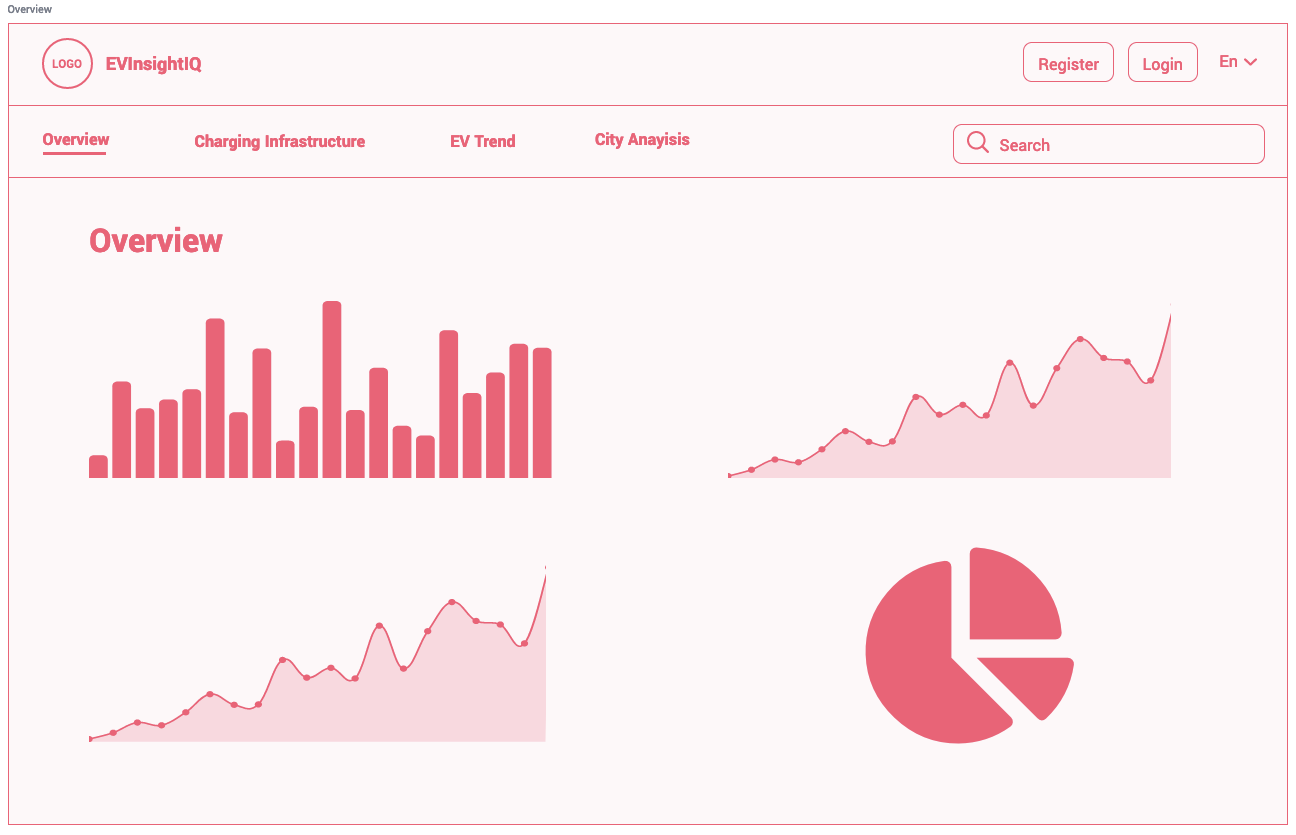
\includegraphics[scale=0.25]{Overview}
    \caption{Overview}
    \label{fig:overview}
\end{figure}

%%%%%%%%%%%%%%%%%%%%%%%%%%%%%%%%%%%%%%%%%%%%%%%%%%%%
% POPULARITY ANALYSIS
%%%%%%%%%%%%%%%%%%%%%%%%%%%%%%%%%%%%%%%%%%%%%%%%%%%%
Finally, we will have a detailed regional popularity analysis page (Figure \ref{fig:city}).
This page will contain detailed information on EV adoption in the states and cities.  Furthermore, one will be able to see a ranking of the
city versus other cities in the state as well as other cities located in other
states.  The user will also be able to compare infrastructure growth and EV
adoption timelines with other cities and the mean adoption rates.
\begin{figure}[h]
    \centering
    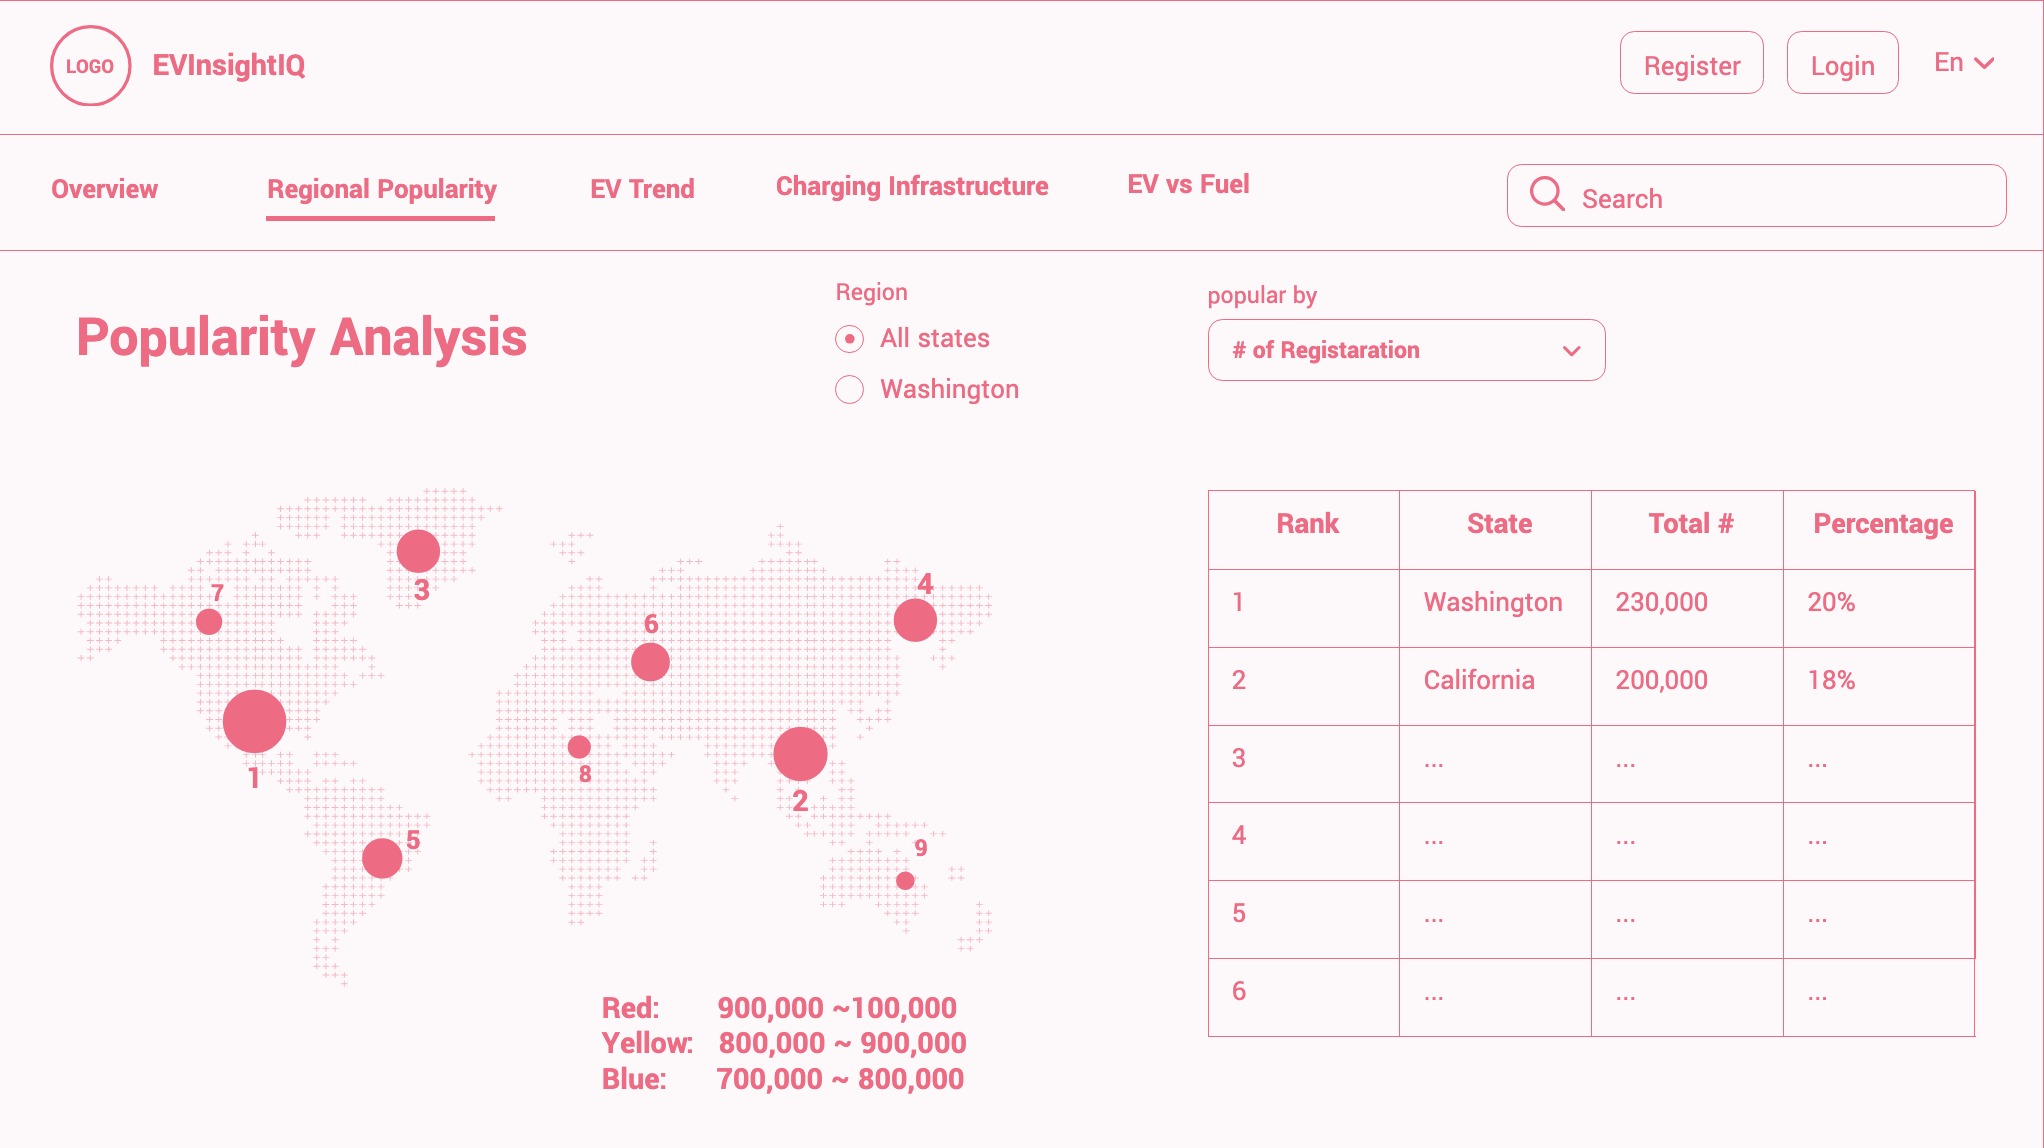
\includegraphics[scale=0.25]{Popularity Analysis}
    \caption{Popularity Analysis}
    \label{fig:city}
\end{figure}

%%%%%%%%%%%%%%%%%%%%%%%%%%%%%%%%%%%%%%%%%%%%%%%%%%%%
% EV TRENDS
%%%%%%%%%%%%%%%%%%%%%%%%%%%%%%%%%%%%%%%%%%%%%%%%%%%%
EV Trends will be able to be seen on this page (Figure \ref{fig:evtrends}).
Some data that will be available on this page, like the infrastructure page, is
the evolution of EV vehicle adoption.  Once again, correlations between other
state adoptions will be able to be visualized with a timeline with laws and
incentives highlighted or tool-tipped.
\begin{figure}[h]
    \centering
    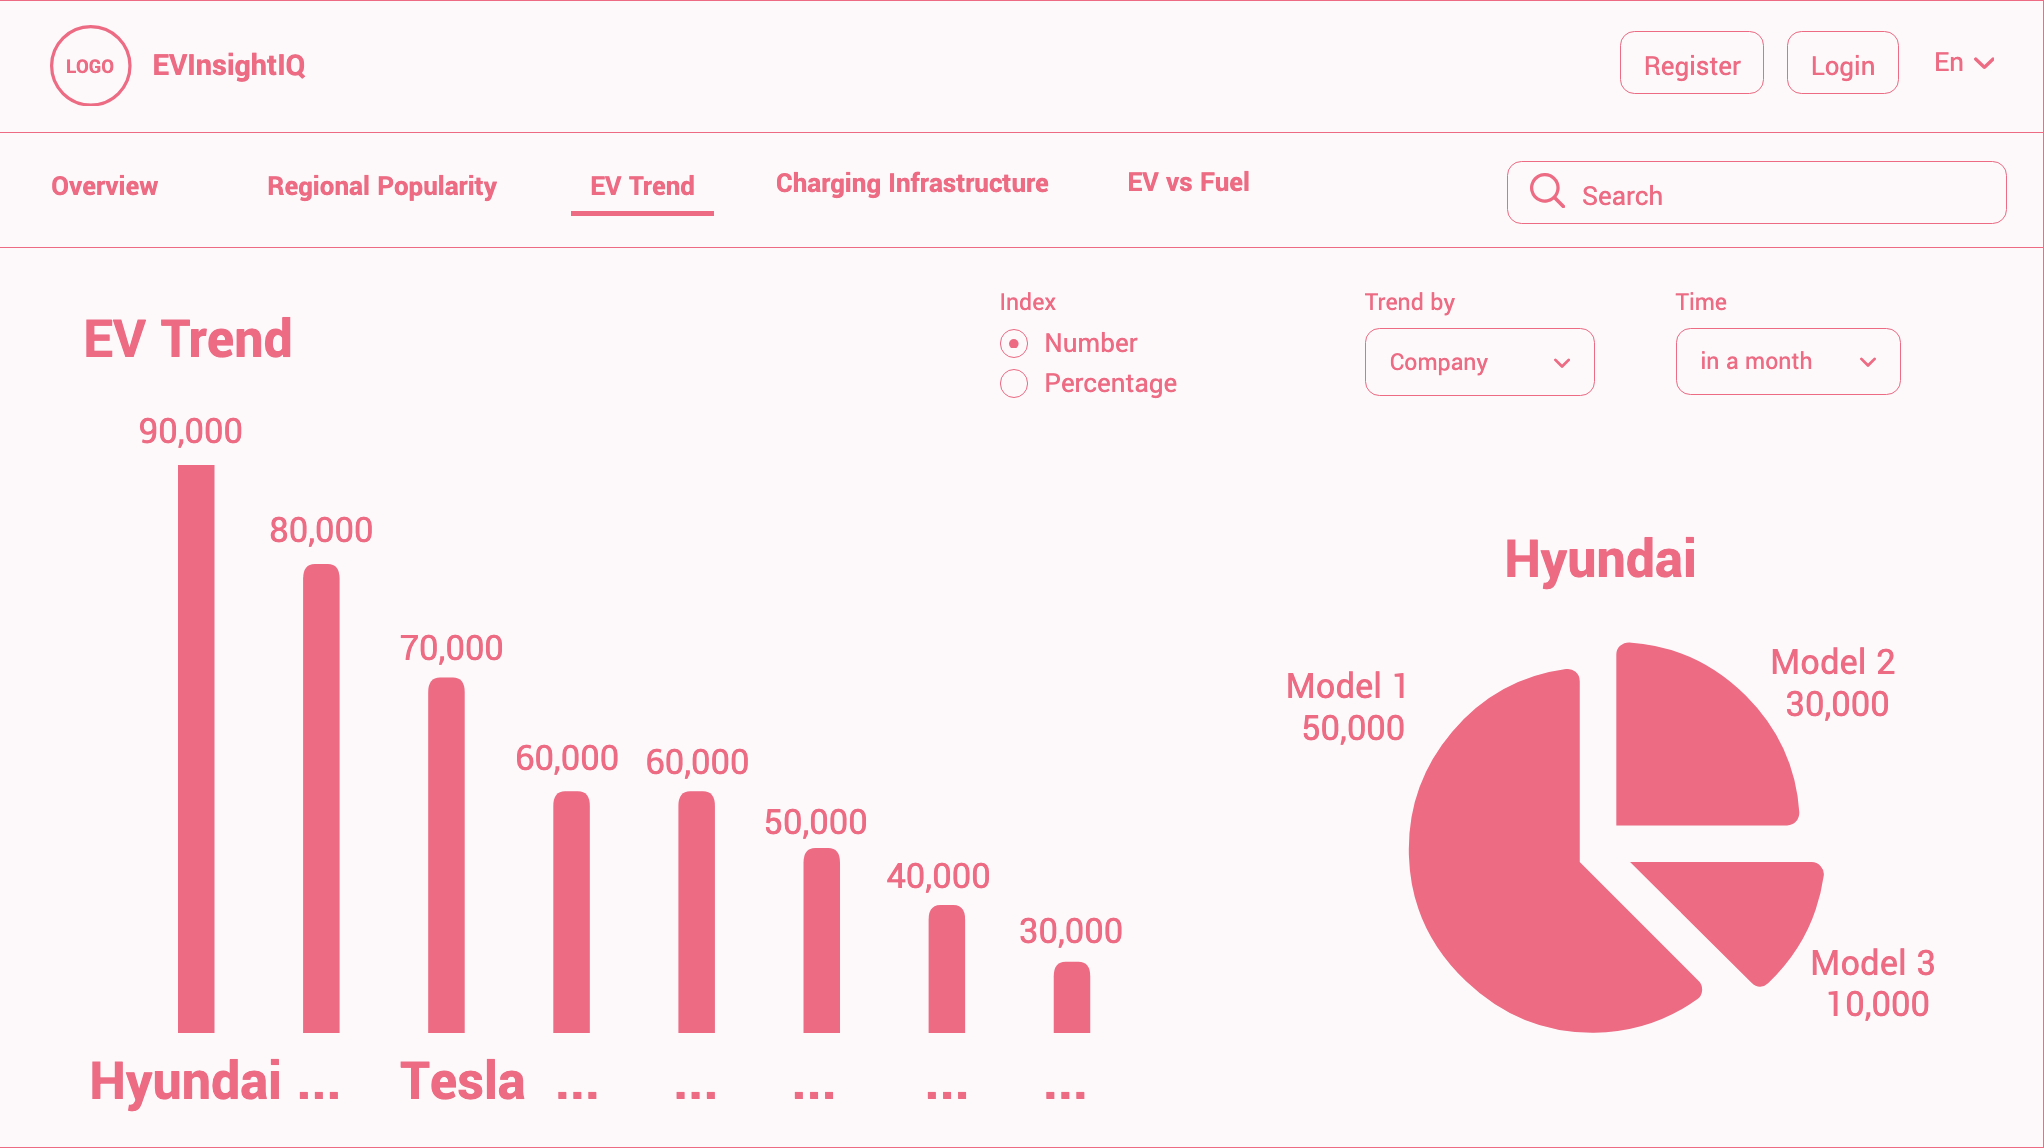
\includegraphics[scale=0.25]{EV Trend}
    \caption{EV Trends}
    \label{fig:evtrends}
\end{figure}

%%%%%%%%%%%%%%%%%%%%%%%%%%%%%%%%%%%%%%%%%%%%%%%%%%%%
% CHARGING INFRASTRUCTURE
%%%%%%%%%%%%%%%%%%%%%%%%%%%%%%%%%%%%%%%%%%%%%%%%%%%%
The second set of visualizations will provide a much deeper look into charging
infrastructure.  On this page (Figure \ref{fig:charge}), the user will be able
to compare the evolution of the charging infrastructure in Washington State and
other states in the US.  Likewise, correlations between different states will be
able to be seen.  Finally, on a timeline graph, the user will be able to see
where legislation was put into effect so that the results can be seen with
respect to those laws and incentives.
\begin{figure}[h]
    \centering
    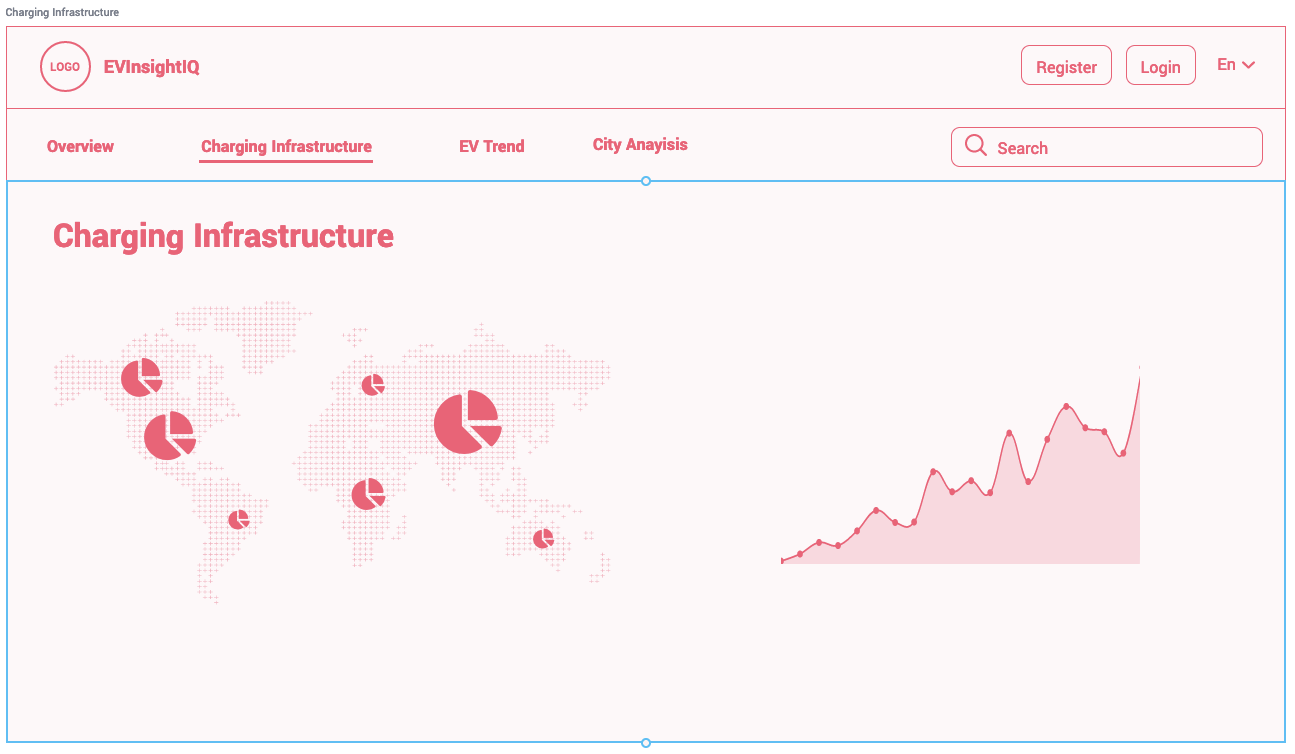
\includegraphics[scale=0.25]{Charging Infrastructure}
    \caption{Charging Infrastructure}
    \label{fig:charge}
\end{figure}

%%%%%%%%%%%%%%%%%%%%%%%%%%%%%%%%%%%%%%%%%%%%%%%%%%%%
% EV vs Fuel
%%%%%%%%%%%%%%%%%%%%%%%%%%%%%%%%%%%%%%%%%%%%%%%%%%%%
EV vs Fuel will be able to be seen on this page (Figure \ref{fig:evfuel}).

\begin{figure}[h]
    \centering
    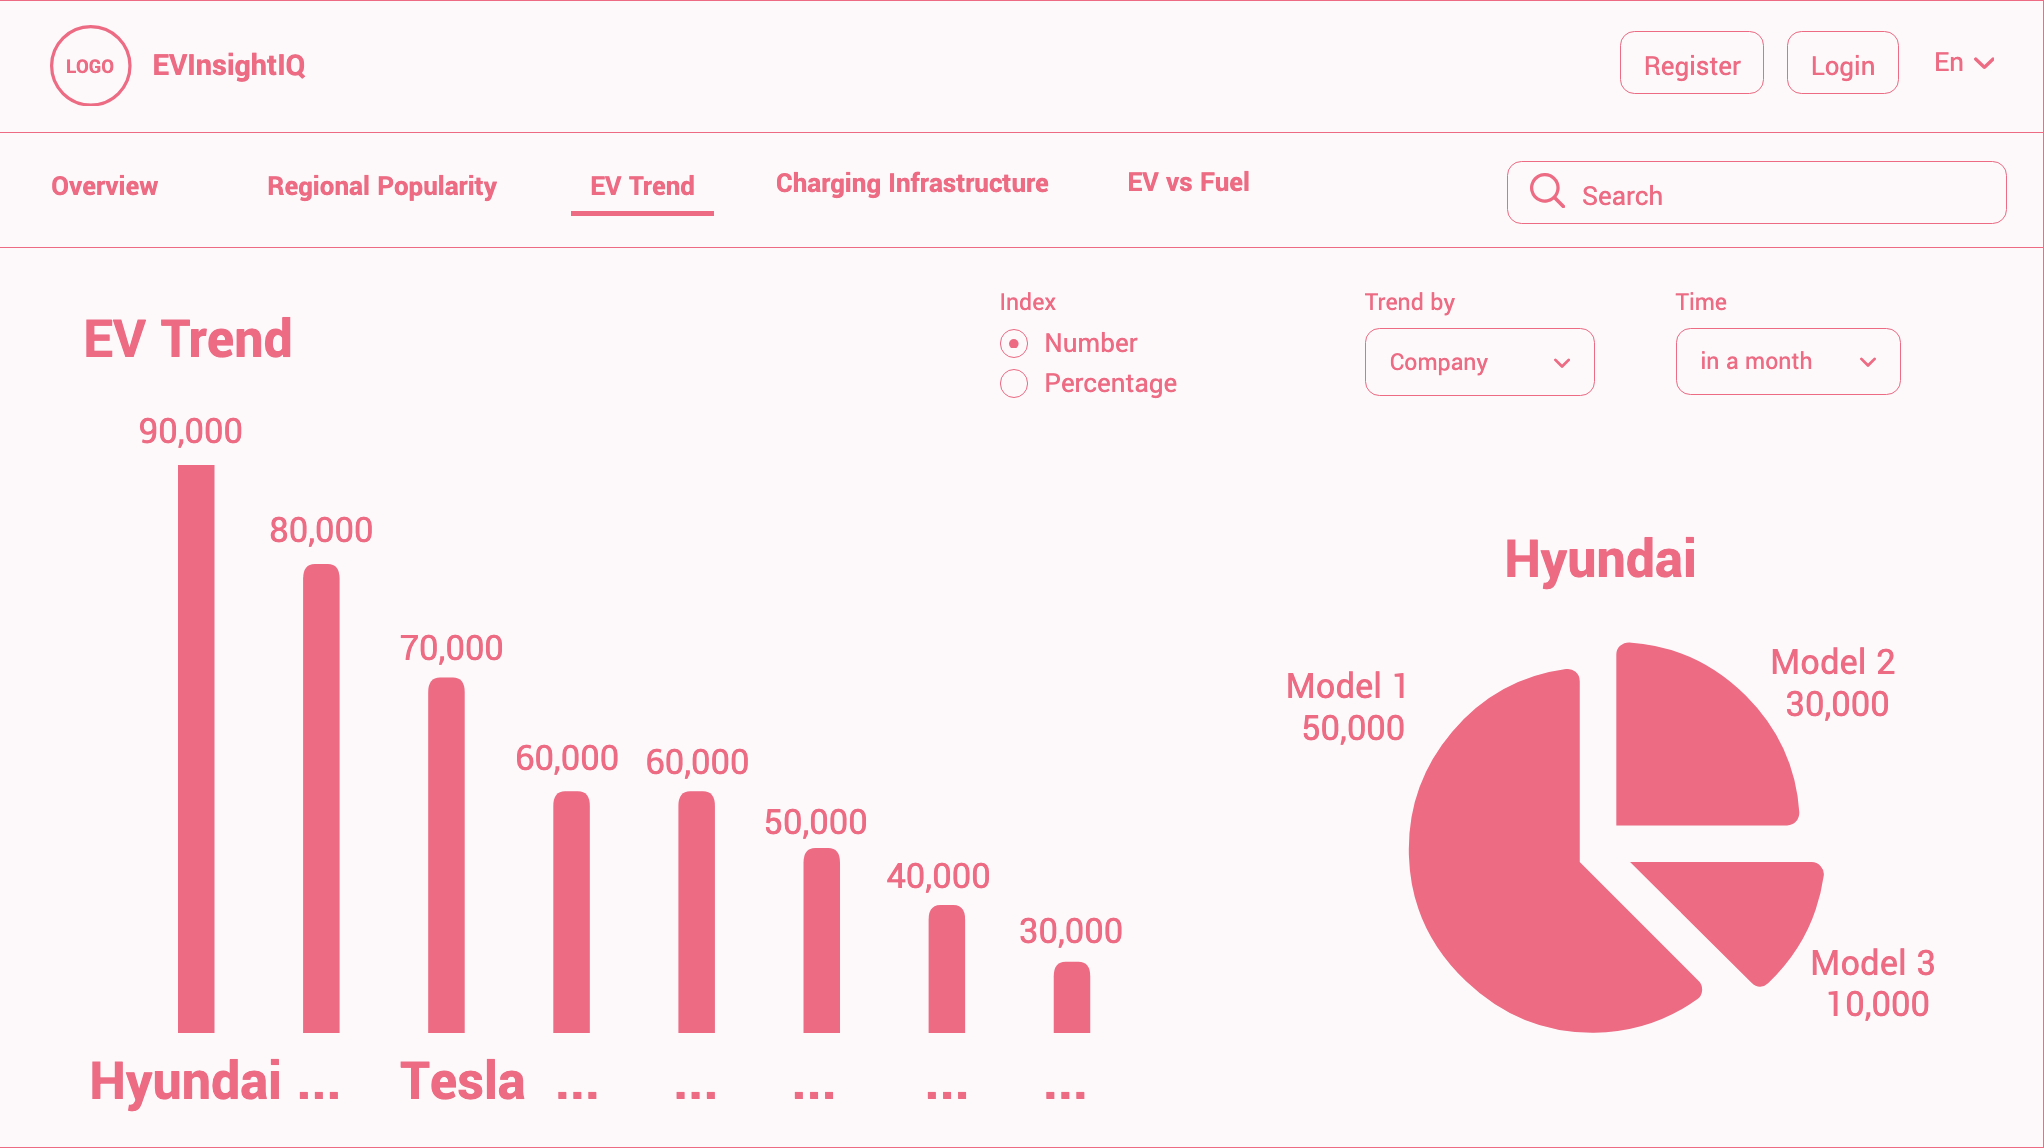
\includegraphics[scale=0.25]{EV Trend}
    \caption{EV vs Fuel}
    \label{fig:evfuel}
\end{figure}

\subsection*{Access to wireframe}
\href{https://claritee.io/view/12733/14589/92396/1bf7a5d4-b9c8-42aa-a914-98842533efbf}{EV data visualization project}\vspace*{5pt}\\

\section*{Data}
\subsection*{Preprocessed and Cleaned}
\href{https://github.com/mk-imagine/csc805g5/tree/main/data}{GitHub Repository of Data}
\subsection*{Source}
\href{https://data.wa.gov/Transportation/Electric-Vehicle-Population-Data/f6w7-q2d2}{Washington State Electric Vehicle Population Data}\vspace*{5pt}\\
\href{https://afdc.energy.gov/data_download}{Alternative Fuel Stations By State (Updated 10-12-2023)}\vspace*{5pt}\\
\href{https://afdc.energy.gov/data_download}{Washington State EV Laws and Incentives}\vspace*{5pt}\\
\href{https://www.atlasevhub.com/materials/state-ev-registration-data/}{EV
Registration Data By State} (This is a massive data set and requires further
cleaning and integration):
\begin{multicols}{4}
    \begin{enumerate}[topsep=0pt, partopsep=0pt, itemsep=1pt, parsep=1pt]
        % \setlength{\itemsep}{0pt}
        % \setlength{\parskip}{0pt}
        \item California
        \item Colorado
        \item Connecticut
        \item Florida
        \item Maine
        \item Minnesota
        \item Montana
        \item New Jersey
        \item New York
        \item North Carolina
        \item Oregon
        \item Tennessee
        \item Texas
        \item Vermont
        \item Virginia
        \item Wisconsin
    \end{enumerate}
\end{multicols}

\section*{Technologies}
\begin{itemize}[topsep=0pt, partopsep=0pt, itemsep=1pt, parsep=1pt, before=\vspace{0pt}]
    \item User Interface (UI): React
    \item Data Visualization: Tableau
    \item Data Source Handling: Incorporating CSV files within the project
    \item Hosting: GitHub for static website hosting
\end{itemize}

\vspace{5mm} %5mm vertical space

We plan to build the website using React, which offers a dynamic and interactive 
web-based environment. For data visualization, We will leverage Tableau, 
a powerful tool known for its effective data representation capabilities. 
To access the data, we will incorporate CSV files directly into the project, 
ensuring easy and seamless data retrieval. 
In terms of hosting, we have chosen to host the static website on GitHub.
These selected technologies and platforms align well with our goal 
for an efficient and engaging visualization system.

\end{document}